%%%%%%%%%%%%%%%%%%%%%%%%%%%%%%%%%%%%%%%%%
% "ModernCV" CV and Cover Letter
% LaTeX Template
% Version 1.2 (25/3/16)
%
% This template has been downloaded from:
% http://www.LaTeXTemplates.com
%
% Original author:
% Xavier Danaux (xdanaux@gmail.com) with modifications by:
% Vel (vel@latextemplates.com)
%
% License:
% CC BY-NC-SA 3.0 (http://creativecommons.org/licenses/by-nc-sa/3.0/)
%
% Important note:
% This template requires the moderncv.cls and .sty files to be in the same 
% directory as this .tex file. These files provide the resume style and themes 
% used for structuring the document.
%
%%%%%%%%%%%%%%%%%%%%%%%%%%%%%%%%%%%%%%%%%

%----------------------------------------------------------------------------------------
%	PACKAGES AND OTHER DOCUMENT CONFIGURATIONS
%----------------------------------------------------------------------------------------

\documentclass[11pt,a4paper,sans]{moderncv} % Font sizes: 10, 11, or 12; paper sizes: a4paper, letterpaper, a5paper, legalpaper, executivepaper or landscape; font families: sans or roman

\moderncvstyle{casual} % CV theme - options include: 'casual' (default), 'classic', 'oldstyle' and 'banking'
\moderncvcolor{blue} % CV color - options include: 'blue' (default), 'orange', 'green', 'red', 'purple', 'grey' and 'black'

\usepackage{lipsum} % Used for inserting dummy 'Lorem ipsum' text into the template
\usepackage{pdfpages}

\usepackage[scale=0.75]{geometry} % Reduce document margins
%\setlength{\hintscolumnwidth}{3cm} % Uncomment to change the width of the dates column
%\setlength{\makecvtitlenamewidth}{10cm} % For the 'classic' style, uncomment to adjust the width of the space allocated to your name

%----------------------------------------------------------------------------------------
%	NAME AND CONTACT INFORMATION SECTION
%----------------------------------------------------------------------------------------

\firstname{Lars} % Your first name
\familyname{Hjerrild} % Your last name

% All information in this block is optional, comment out any lines you don't need
\title{Curriculum Vitae}
\address{Jens Baggesensvej 118, 8200}{Aarhus N, Danmark}
\mobile{(+45) 42 42 08 83}
\phone{(None) }
%\fax{(000) 111 1113}
\email{larshjerrild@hotmail.com}
%\homepage{staff.org.edu/~jsmith}{staff.org.edu/$\sim$jsmith} % The first argument is the url for the clickable link, the second argument is the url displayed in the template - this allows special characters to be displayed such as the tilde in this example
%\extrainfo{additional information}
\photo[70pt][0.4pt]{pictures/picture} % The first bracket is the picture height, the second is the thickness of the frame around the picture (0pt for no frame)
%\quote{"T" - John Smith}

%----------------------------------------------------------------------------------------

\begin{document}

%----------------------------------------------------------------------------------------
%	COVER LETTER
%----------------------------------------------------------------------------------------

% To remove the cover letter, comment out this entire block

%\clearpage
%
%\recipient{HR Department}{Corporation\\123 Pleasant Lane\\12345 City, State} % Letter recipient
%\date{\today} % Letter date
%\opening{Dear Sir or Madam,} % Opening greeting
%\closing{Sincerely yours,} % Closing phrase
%\enclosure[Attached]{curriculum vit\ae{}} % List of enclosed documents
%
%\makelettertitle % Print letter title
%
%\lipsum[1-3] % Dummy text
%
%\makeletterclosing % Print letter signature
%

\textbf{Ans\o gning  vedr. praktikstilling i Systematic}



\vspace{3mm}
Med venlig hilsen

\vspace{5mm}
Lars Hjerrild



\vspace{8mm}
Bilag : CV og Karakterudskrift 







\newpage

%----------------------------------------------------------------------------------------
%	CURRICULUM VITAE
%----------------------------------------------------------------------------------------

\makecvtitle % Print the CV title

%----------------------------------------------------------------------------------------
%	EDUCATION SECTION
%----------------------------------------------------------------------------------------

\section{Om mig}
Personligt bruger jeg tid p\aa at tr\ae ne, fordi jeg elsker at komme ud at bev\ae ge mig. Fx Som det er nu spiller jeg fast hockey et par timer om ugen. Jeg har som teenager (15-20) gået rigtig meget op i sporten orienteringsløb, hvor jeg i fire år var en del af det danske juniorlandshold. Jeg har derigennem lært meget om at arbejde struktureret til at blive bedre, og hvor stor en betydning det milj\o man arbejder i har. Jeg er som person en smule stille og meget analytisk, men alligevel g\aa r jeg meget op i at folk har det godt, og den derv\ae rende juniorlandstr\ae ner sagde ogs\aa til mig da jeg stoppede at han aldrig har haft en l\oe ber der havde givet ham s\aa mange high fives. Jeg kan godt lide at fejre succeser og har derudover interesse i musik og er i \oe vrigt ret god til engelsk da jeg har boet i USA i et \aa r, og g\aa et p\aa en amerikansk elementary school. Jeg har s\aa gar et amerikansk mesterskab i M12 i orienteringsl\o b 

\section{Uddannelse}

\cventry{2015--2018}{DiplomIngeni\o r i information og kommunikationsteknologi}{Aarhus Universitet}{IHA}
{}{}  % Arguments not required can be left empty
\cventry{2010--2014}{Stx}{Marselisborg Gymnasium}{}
{}{}
\cventry{2009--2010}{Efterskole}{himmelbjergegnens natur og idr\a tsefterskole}{}
{}{}

%\section{Masters Thesis}
%\cvitem{Title}{\emph{Money Is The Root Of All Evil -- Or Is It?}}
%\cvitem{Supervisors}{Professor James Smith \& Associate Professor Jane Smith}
%\cvitem{Description}{This thesis explored the idea that money has been the cause of untold anguish and suffering in the world. I found that it has, in fact, not.}


%----------------------------------------------------------------------------------------
%	WORK EXPERIENCE SECTION
%----------------------------------------------------------------------------------------

\section{Erfaring}

Arbejdede i en kort periode som vikar, hvor jeg hjalp som lagerarbejder. Det hjalp til at sparre lidt sm\aa knaster op til at komme ud og rejse. 
%
%\subsection{Vocational}
%
%\cventry{2012--Present}{1\textsuperscript{st} Year Analyst}{\textsc{Lehman Brothers}}{Los Angeles}{}{Developed spreadsheets for risk analysis on exotic derivatives on a wide array of commodities (ags, oils, precious and base metals), managed blotter and secondary trades on structured notes, liaised with Middle Office, Sales and Structuring for bookkeeping.
%\newline{}\newline{}
%Detailed achievements:
%\begin{itemize}
%\item Learned how to make amazing coffee
%\item Finally determined the reason for \textsc{PC LOAD LETTER}:
%\begin{itemize}
%\item Paper jam
%\item Software issues:
%\begin{itemize}
%\item Word not sending the correct data to printer
%\item Windows trying to print in letter format
%\end{itemize}
%\item Coffee spilled inside printer
%\end{itemize}
%\item Broke the office record for number of kitten pictures in cubicle
%\end{itemize}}

%------------------------------------------------

%\cventry{2010--2011}{Summer Intern}{\textsc{Lehman Brothers}}{Los Angeles}{}{Rated "truly distinctive" for Analytical Skills and Teamwork.}

%------------------------------------------------
%
\subsection{Diverse}

Jeg har efterh\aa nden mange gange arrangeret l\o b og tr\ae ning hvor jeg uden fastans\ae ttelse har tjent penge både til mig selv eller til min egen klub(Orienteringsl\o b).

%
%\cventry{2008--2009}{Computer Repair Specialist}{Buy More}{Burbank}{}{Worked in the Nerd Herd and helped to solve computer problems by asking customers to turn their computers off and on again.}

%----------------------------------------------------------------------------------------
%	AWARDS SECTION
%----------------------------------------------------------------------------------------
%
%\section{Om mig}
%
%\cvitem{2011}{School of Business Postgraduate Scholarship}
%\cvitem{2010}{Top Achiever Award -- Commerce}

%----------------------------------------------------------------------------------------
%	COMPUTER SKILLS SECTION
%----------------------------------------------------------------------------------------

\section{Faglig kompetancer}

\cvitem{}{\textsc{C}    \textsc{C++}  \textsc{C\#}}
\cvitem{}{\textsc{Bootstrap} \textsc{CSS} \textsc{Git}  \textsc{HTML5} \textsc{Linux} }


%----------------------------------------------------------------------------------------
%	COMMUNICATION SKILLS SECTION
%----------------------------------------------------------------------------------------
%
%\section{Communication Skills}
%
%\cvitem{2010}{Oral Presentation at the California Business Conference}
%\cvitem{2009}{Poster at the Annual Business Conference in Oregon}

%----------------------------------------------------------------------------------------
%	LANGUAGES SECTION
%----------------------------------------------------------------------------------------

%----------------------------------------------------------------------------------------
%	INTERESTS SECTION
%----------------------------------------------------------------------------------------

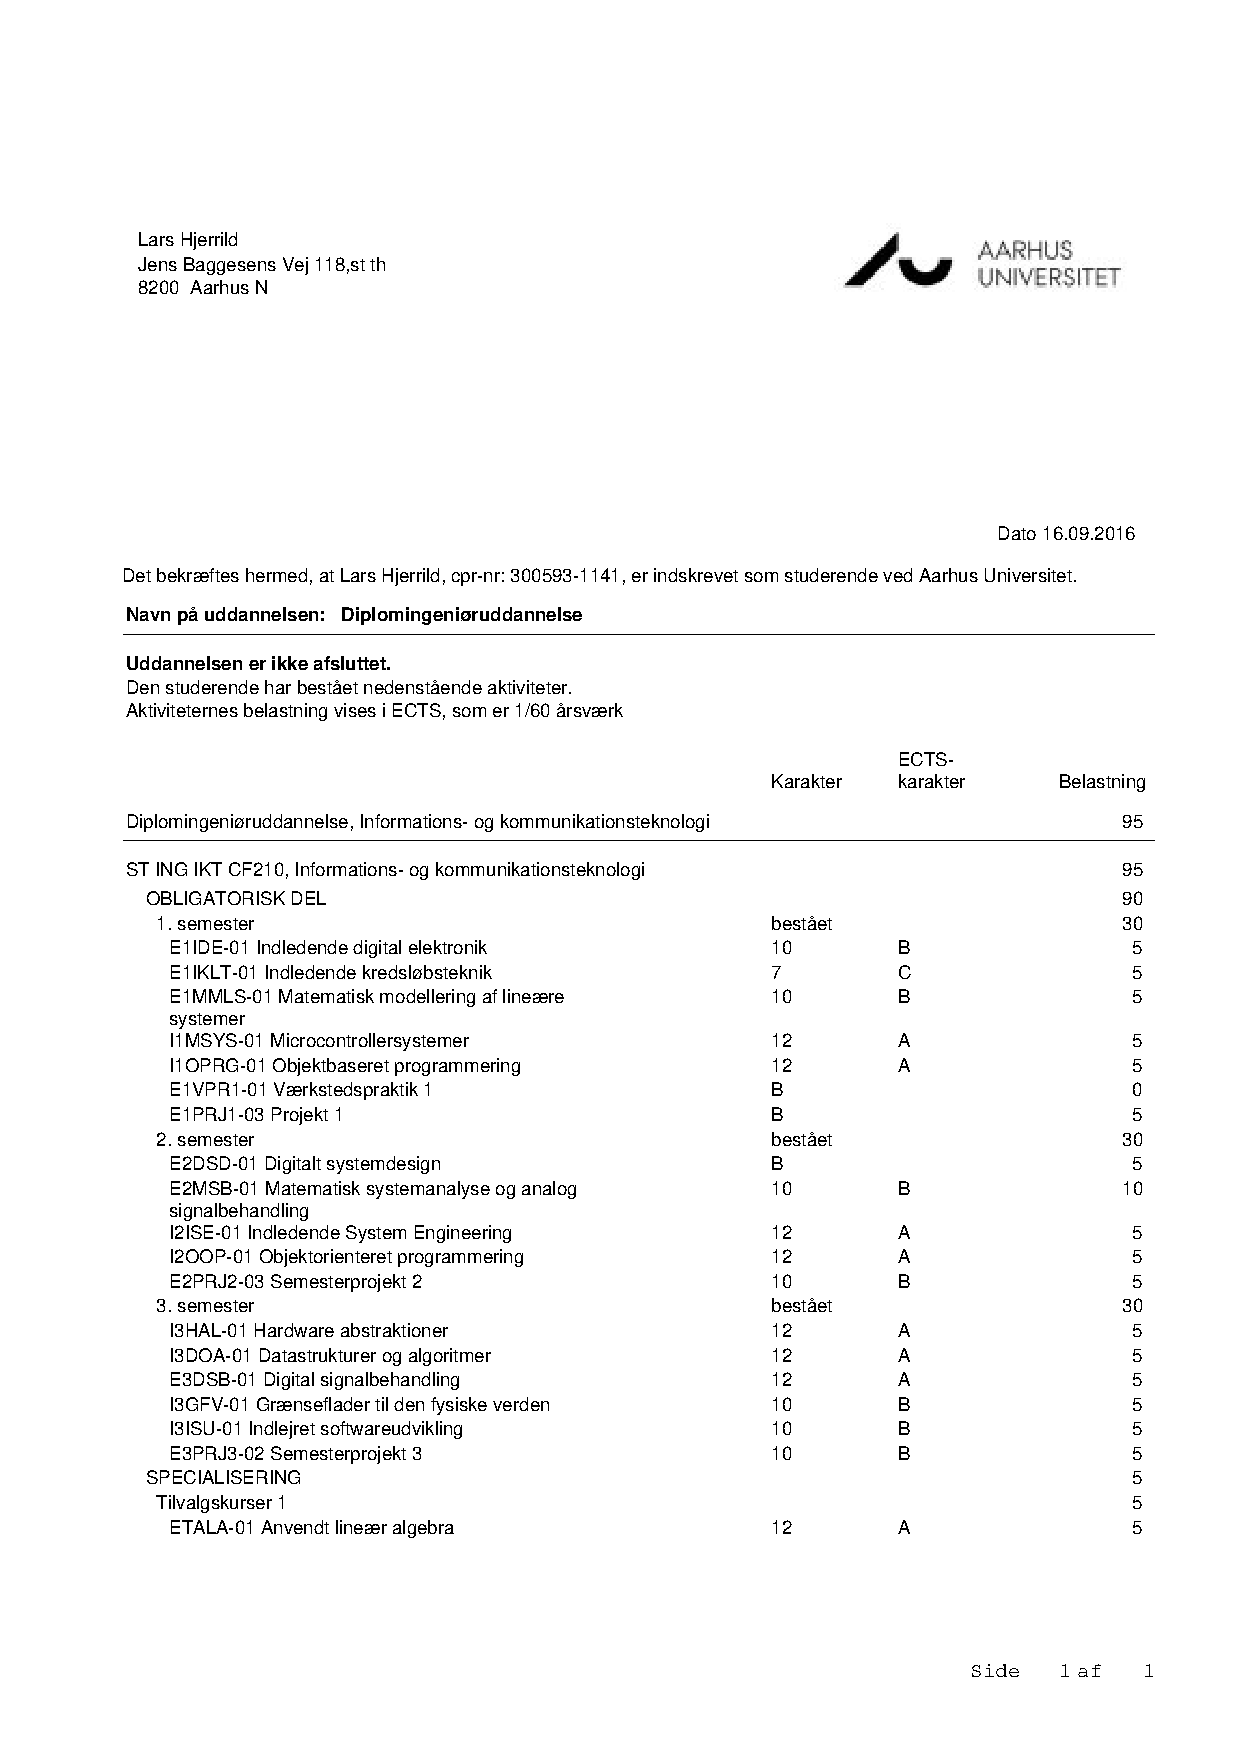
\includepdf[pages={1}]{pictures/Karakterudskrift.pdf}

%----------------------------------------------------------------------------------------

\end{document}